\section{Chainball (60pts)}
如图\ref{fig:chainball} 所示,一个简单的链条球模型由三个质量为$m$的球体和两根无质量的轻绳组成。现在固定最上方的一个球体,并自然下垂。绳子的长度均为\(l\), 重力加速度为\(g\).

\begin{figure}
	\centering
	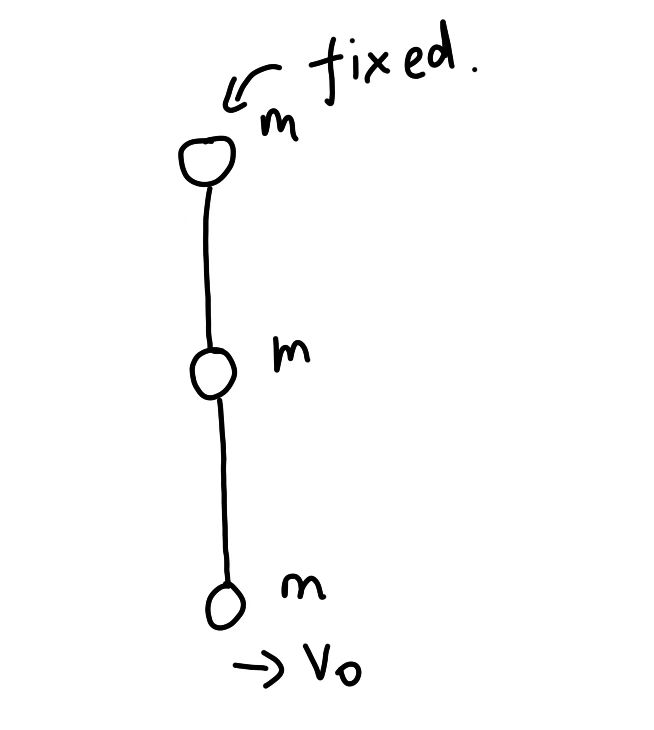
\includegraphics[width=0.3\textwidth]{chainball}
	\caption{三个质量为$m$的球体由两根无质量的轻绳连接成链条球模型,最上方的球体固定.}
	\label{fig:chainball}
\end{figure}

\begin{enumerate}
	\item 现在突然给予最下方的球体一个向右的初速度$v_0$,求出最下方球体的水平方向上的位移随时间变化的关系式。(设\(v_{0}\)很小可以视为小振动)(30pts)
	\item 在第一小问的设定下,最下方球体水平方向上最远可以达到的位移是多少?(4pts)
	\item 现在只限制下方小球的初速度为向右的初速度为\(v_0\),请问是否有方式使得摆动看起来“更有规律”?即:每次当中间球体回到最低点时,最下方的球体也回到最低点。如果有,请给出所有还需要的条件;如果没有,请给出理由。(16ps)
	\item 下面考虑一个更复杂一点的情况:现在由\(n+2\)个质量为\(m\)的球体组成类似的链条球模型。如图\ref{fig:chainball2}所示。为了更容易计算,现设定如下:初始时上方\(n\)个球均是固定的,只有最下方两个球可以自由移动,仍然给予最下方球初速度\(v_{0}\),当倒数第二个球体再次回到最低点的时刻,通过Teyvat的神秘力量使得最后一根绳子断裂(即编号为0的球体会脱落),同时解除编号为2的球体的锁定。如此递推,每次保持只有两个球体会活动,直到只剩下编号为\(n\)与\(n+1\)的球体。请求出此时编号为\(n\)的球体的水平方向上的位移随时间变化的关系式。(\(v_{0}\)仍然认为只能引起小振动)(10pts)
	\begin{figure}[htbp]
	\centering
	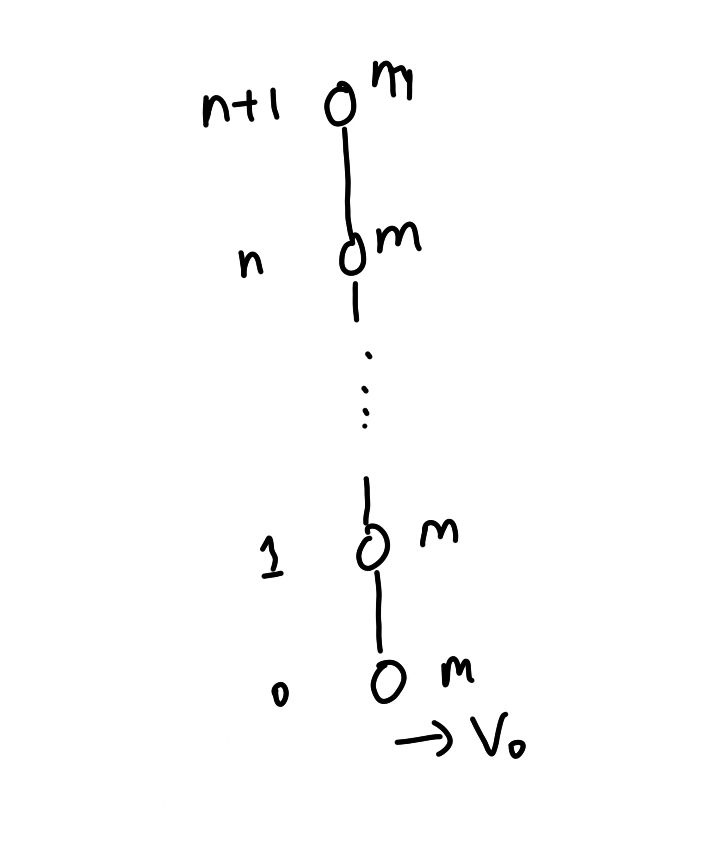
\includegraphics[width=0.3\textwidth]{chainball2}
	\caption{多级链条球.}
	\label{fig:chainball2}
 \end{figure}
\end{enumerate}